\documentclass[11pt]{article}

\usepackage[margin=1in]{geometry}
\usepackage{hyperref}
\usepackage{booktabs}
\usepackage{url}
\usepackage{amssymb}
\usepackage{amsmath}
\usepackage{natbib}
\usepackage{microtype}
\usepackage{listings}
\usepackage{graphicx}
\usepackage{xcolor}
\usepackage{placeins}

\lstset{
  basicstyle=\small\ttfamily,
  breaklines=true,
  frame=single,
  language=Python,
  numbers=left,
  numberstyle=\tiny\color{gray},
  xleftmargin=2em,
  showstringspaces=false,
}

\title{Endgame: A Unified Framework for Modern Machine Learning Workflows}

\author{
  Cameron Hamilton \\
  Alliance AI \\
  \texttt{cameron@allianceai.co}
}

\date{}

\begin{document}

\maketitle

\begin{abstract}
Modern ML workflows require integrating disparate libraries---each with its
own interface, data format, and installation path---making fair comparison
across model families unnecessarily difficult. To bridge this gap, we present
\textsc{Endgame}, an open-source Python framework that unifies classic and
modern methods under a single scikit-learn-compatible API. The framework
spans supervised learning (gradient boosted trees, deep tabular
architectures, interpretable glass-box models), uncertainty quantification
(conformal prediction, Venn-ABERS calibration), ensemble optimization, and
domain-specific modules for time series, signal processing, and multimodal
data. Endgame provides 33 interpretable models across 9 paradigms under
one API, a built-in Model Context Protocol (MCP) server enabling LLM agents
to construct complete pipelines through natural language, and a 15-stage
AutoML pipeline with quality guardrails and automatic calibration. We
validate these capabilities across 29 benchmark datasets and 49 models.
The software is available under the Apache~2.0 license at
\url{https://github.com/allianceai/endgame}.
\end{abstract}

\noindent\textbf{Keywords:}
Machine Learning, Open Source Software, Scikit-learn, Tabular Data,
Ensemble Methods, Conformal Prediction, Interpretable Machine Learning

%% --------------------------------------------------------------------------
\section{Introduction}
\label{sec:intro}

Machine learning research and deployment today require stitching together
dozens of libraries with incompatible APIs. A researcher comparing a
LightGBM ensemble against an Explainable Boosting Machine and a conformal
predictor backed by a FT-Transformer must navigate three different installation
paths, three different calling conventions, and three different output
formats---before even reaching the modeling question they set out to answer.
This fragmentation slows iteration, hinders reproducibility, and makes fair
comparison across model families unnecessarily difficult.

The problem is compounded as practitioners move from research to production.
Models that performed well in notebooks must be re-wrapped for calibration,
constraint checking, and deployment---typically requiring yet another layer
of library-specific glue code.

\textsc{Endgame} addresses this with a single framework where every
component---from a LightGBM wrapper to a Bayesian Model Averaging ensemble
to a wavelet packet transformer---implements the scikit-learn
\texttt{fit}/\texttt{predict}/\texttt{transform} interface. The framework
spans tabular, time series, signal processing, computer vision, NLP, and
audio domains, though the core emphasis is on tabular learning where the
unification benefit is greatest.

The primary contribution is a unified ML framework with first-class support
for interpretable and calibrated models. The library makes five specific
contributions:

\begin{enumerate}
\item \textbf{API unification across model families.} Endgame wraps
  supervised models---gradient boosted trees, deep tabular architectures,
  Bayesian classifiers, rule learners, interpretable glass-box models, and
  domain-specific methods---under a consistent scikit-learn interface.
  Switching from a black-box LightGBM to a hand-scoreable risk scorecard
  requires changing one line of code.

\item \textbf{Interpretable models as first-class citizens.} 33 glass-box
  models spanning GAMs (EBM, pyGAM, GAMI-Net, NODE-GAM, NAM), optimal rule
  systems (CORELS, GOSDT), integer risk scorecards (SLIM, FasterRisk),
  symbolic regression (PySR), and fuzzy rules (FURIA)---all sharing the
  same interface as black-box models, enabling direct comparison of
  accuracy--interpretability trade-offs within a single experiment.

\item \textbf{Rigorous uncertainty quantification.} Conformal prediction
  for classification and regression, Venn-ABERS probability calibration,
  and conformalized quantile regression---providing distribution-free
  coverage guarantees largely absent from general-purpose ML toolkits.

\item \textbf{LLM-driven pipeline construction.} A built-in Model Context
  Protocol (MCP) server \citep{anthropic2024mcp} that enables LLM agents to
  build complete ML pipelines through natural language conversation---to our
  knowledge, the first ML toolkit with native MCP integration.

\item \textbf{Production-grade AutoML.} A 15-stage AutoML pipeline with
  quality guardrails, deployment constraints, and automatic calibration
  that goes beyond the standard train--evaluate--ensemble loop.
\end{enumerate}

%% --------------------------------------------------------------------------
\section{Design Philosophy}
\label{sec:design}

Endgame is organized around three principles that guided its architecture.

\paragraph{Strict sklearn compatibility.} Every estimator implements
\texttt{fit}, \texttt{predict}, and where applicable \texttt{predict\_proba},
\texttt{transform}, and \texttt{feature\_importances\_}. This is not merely
a convention: Endgame models must pass scikit-learn's
\texttt{check\_estimator} suite and work as drop-in replacements within
\texttt{Pipeline}, \texttt{GridSearchCV}, and \texttt{cross\_val\_score}.
The practical consequence is that users can mix Endgame components with any
existing sklearn pipeline without adapter code.

\paragraph{Composability across model families.} A key design goal is that
any estimator can be combined with any ensemble method, any calibration
wrapper, and any cross-validation strategy. An EBM can serve as a base
learner in a Super Learner ensemble, which can be wrapped in a conformal
predictor, which can be evaluated with combinatorial purged cross-validation
for financial backtesting---all using the same API. This composability
emerges from the strict interface contract rather than from special-case
integration.

\paragraph{Research-to-production continuum.} Rather than treating research
experimentation and production deployment as separate concerns, Endgame
provides a continuous workflow. The same model used in a benchmark can be
wrapped with conformal prediction intervals, subjected to deployment
constraints (latency, model size, interpretability requirements), exported
to ONNX, and served---without reimplementation. The AutoML module enforces
this continuum by including guardrail, calibration, and constraint-checking
stages alongside the standard train--evaluate--ensemble loop.

%% --------------------------------------------------------------------------
\section{Software Description}
\label{sec:software}

\subsection{Architecture}

Endgame is organized into 27 Python submodules following the ML workflow
(Table~\ref{tab:modules}). Core dependencies are minimal (NumPy, Polars,
scikit-learn, Optuna, SciPy); domain-specific backends (PyTorch, LightGBM,
statsforecast, librosa) are optional and lazily imported, keeping
\texttt{import endgame} fast ($<$0.5s) for lightweight workflows.

\begin{table}[h]
\centering
\caption{Module overview. Component counts are approximate; several modules
  include additional utility classes not listed here.}
\label{tab:modules}
\small
\begin{tabular}{@{}ll@{}}
\toprule
\textbf{Module} & \textbf{Scope} \\
\midrule
\texttt{models}        & Supervised estimators: GBDTs, deep tabular, trees, rules, Bayesian, kernel, interpretable \\
\texttt{preprocessing} & Encoding, imputation, imbalanced learning (25 samplers), noise detection \\
\texttt{ensemble}      & Voting, bagging, boosting, stacking, Super Learner, BMA, NCL \\
\texttt{calibration}   & Conformal prediction, Venn-ABERS, temperature/Platt/beta/isotonic scaling \\
\texttt{validation}    & 8 CV strategies, adversarial validation, drift detection \\
\texttt{signal}        & Filtering, spectral analysis, wavelets, entropy, complexity, spatial \\
\texttt{timeseries}    & Forecasting (statistical + neural), ROCKET/HYDRA classification \\
\texttt{visualization} & Self-contained interactive HTML charts and model evaluation reports \\
\texttt{automl}        & Multi-stage AutoML: profiling, guardrails, HPO, constraints, calibration \\
\texttt{anomaly}       & Isolation Forest, LOF, GritBot, PyOD wrapper \\
\texttt{explain}       & SHAP, LIME, PDP, feature interactions, counterfactuals \\
\texttt{fairness}      & Fairness metrics, bias mitigation, group calibration \\
\texttt{tracking}      & Experiment logging (MLflow, console) \\
\texttt{mcp}           & Model Context Protocol server for LLM integration \\
\bottomrule
\end{tabular}
\end{table}

\paragraph{Polars-first preprocessing.} Tabular transformers convert inputs
to \texttt{pl.LazyFrame} internally, achieving 2--10$\times$ speedups over
pandas for aggregation and encoding operations, while transparently accepting
NumPy and pandas inputs.

\subsection{Notable Components}

\paragraph{Conformal prediction.} \texttt{ConformalClassifier} and
\texttt{ConformalRegressor} implement split conformal inference with
exchangeability-based guarantees. \texttt{ConformizedQuantileRegressor}
provides adaptive-width intervals via CQR \citep{romano2019conformalized}.

\paragraph{Deep tabular models.} Wrappers for FT-Transformer
\citep{gorishniy2021revisiting}, SAINT \citep{somepalli2021saint},
TabPFN \citep{hollmann2022tabpfn}, NODE \citep{popov2020neural},
GRANDE \citep{marton2024grande}, and TabR \citep{gorishniy2024tabr},
all with consistent \texttt{fit}/\texttt{predict} APIs and competition-tuned
default hyperparameters.

\paragraph{Super Learner.} Implements the optimal convex combination of
base learners via non-negative least squares on out-of-fold predictions
\citep{van2007super}, with optional ridge meta-learning.

\paragraph{Interpretable models.} Endgame provides a broad suite of
glass-box models spanning multiple interpretability paradigms:
\emph{additive models} (EBM \citep{nori2019interpretml}, pyGAM, GAMI-Net,
NODE-GAM, NAM) decompose predictions into per-feature shape functions;
\emph{optimal rule systems} (CORELS \citep{angelino2017learning}, GOSDT
\citep{lin2020generalized}) provide provably optimal rule lists and sparse
decision trees; \emph{risk scorecards} (SLIM, FasterRisk
\citep{liu2022fasterrisk}) produce hand-scoreable integer coefficients for
clinical and regulatory settings; and \emph{symbolic regression} (PySR
\citep{cranmer2023interpretable}) discovers closed-form equations. All share
the same \texttt{fit}/\texttt{predict} interface as black-box models.

\paragraph{AutoML pipeline.} The \texttt{automl} module provides a
multi-stage pipeline orchestrated by a time-budget manager with dynamic
reallocation. Beyond the standard profiling--training--ensembling loop,
the pipeline includes quality guardrails that detect target leakage and
data health issues before training begins, Optuna-based hyperparameter
tuning of the top-$k$ models, deployment constraint checking that validates
latency and model size requirements, threshold optimization on out-of-fold
predictions, and a SHAP-based explainability stage. Six presets control
the quality--speed trade-off.

\begin{figure}[!htb]
\centering
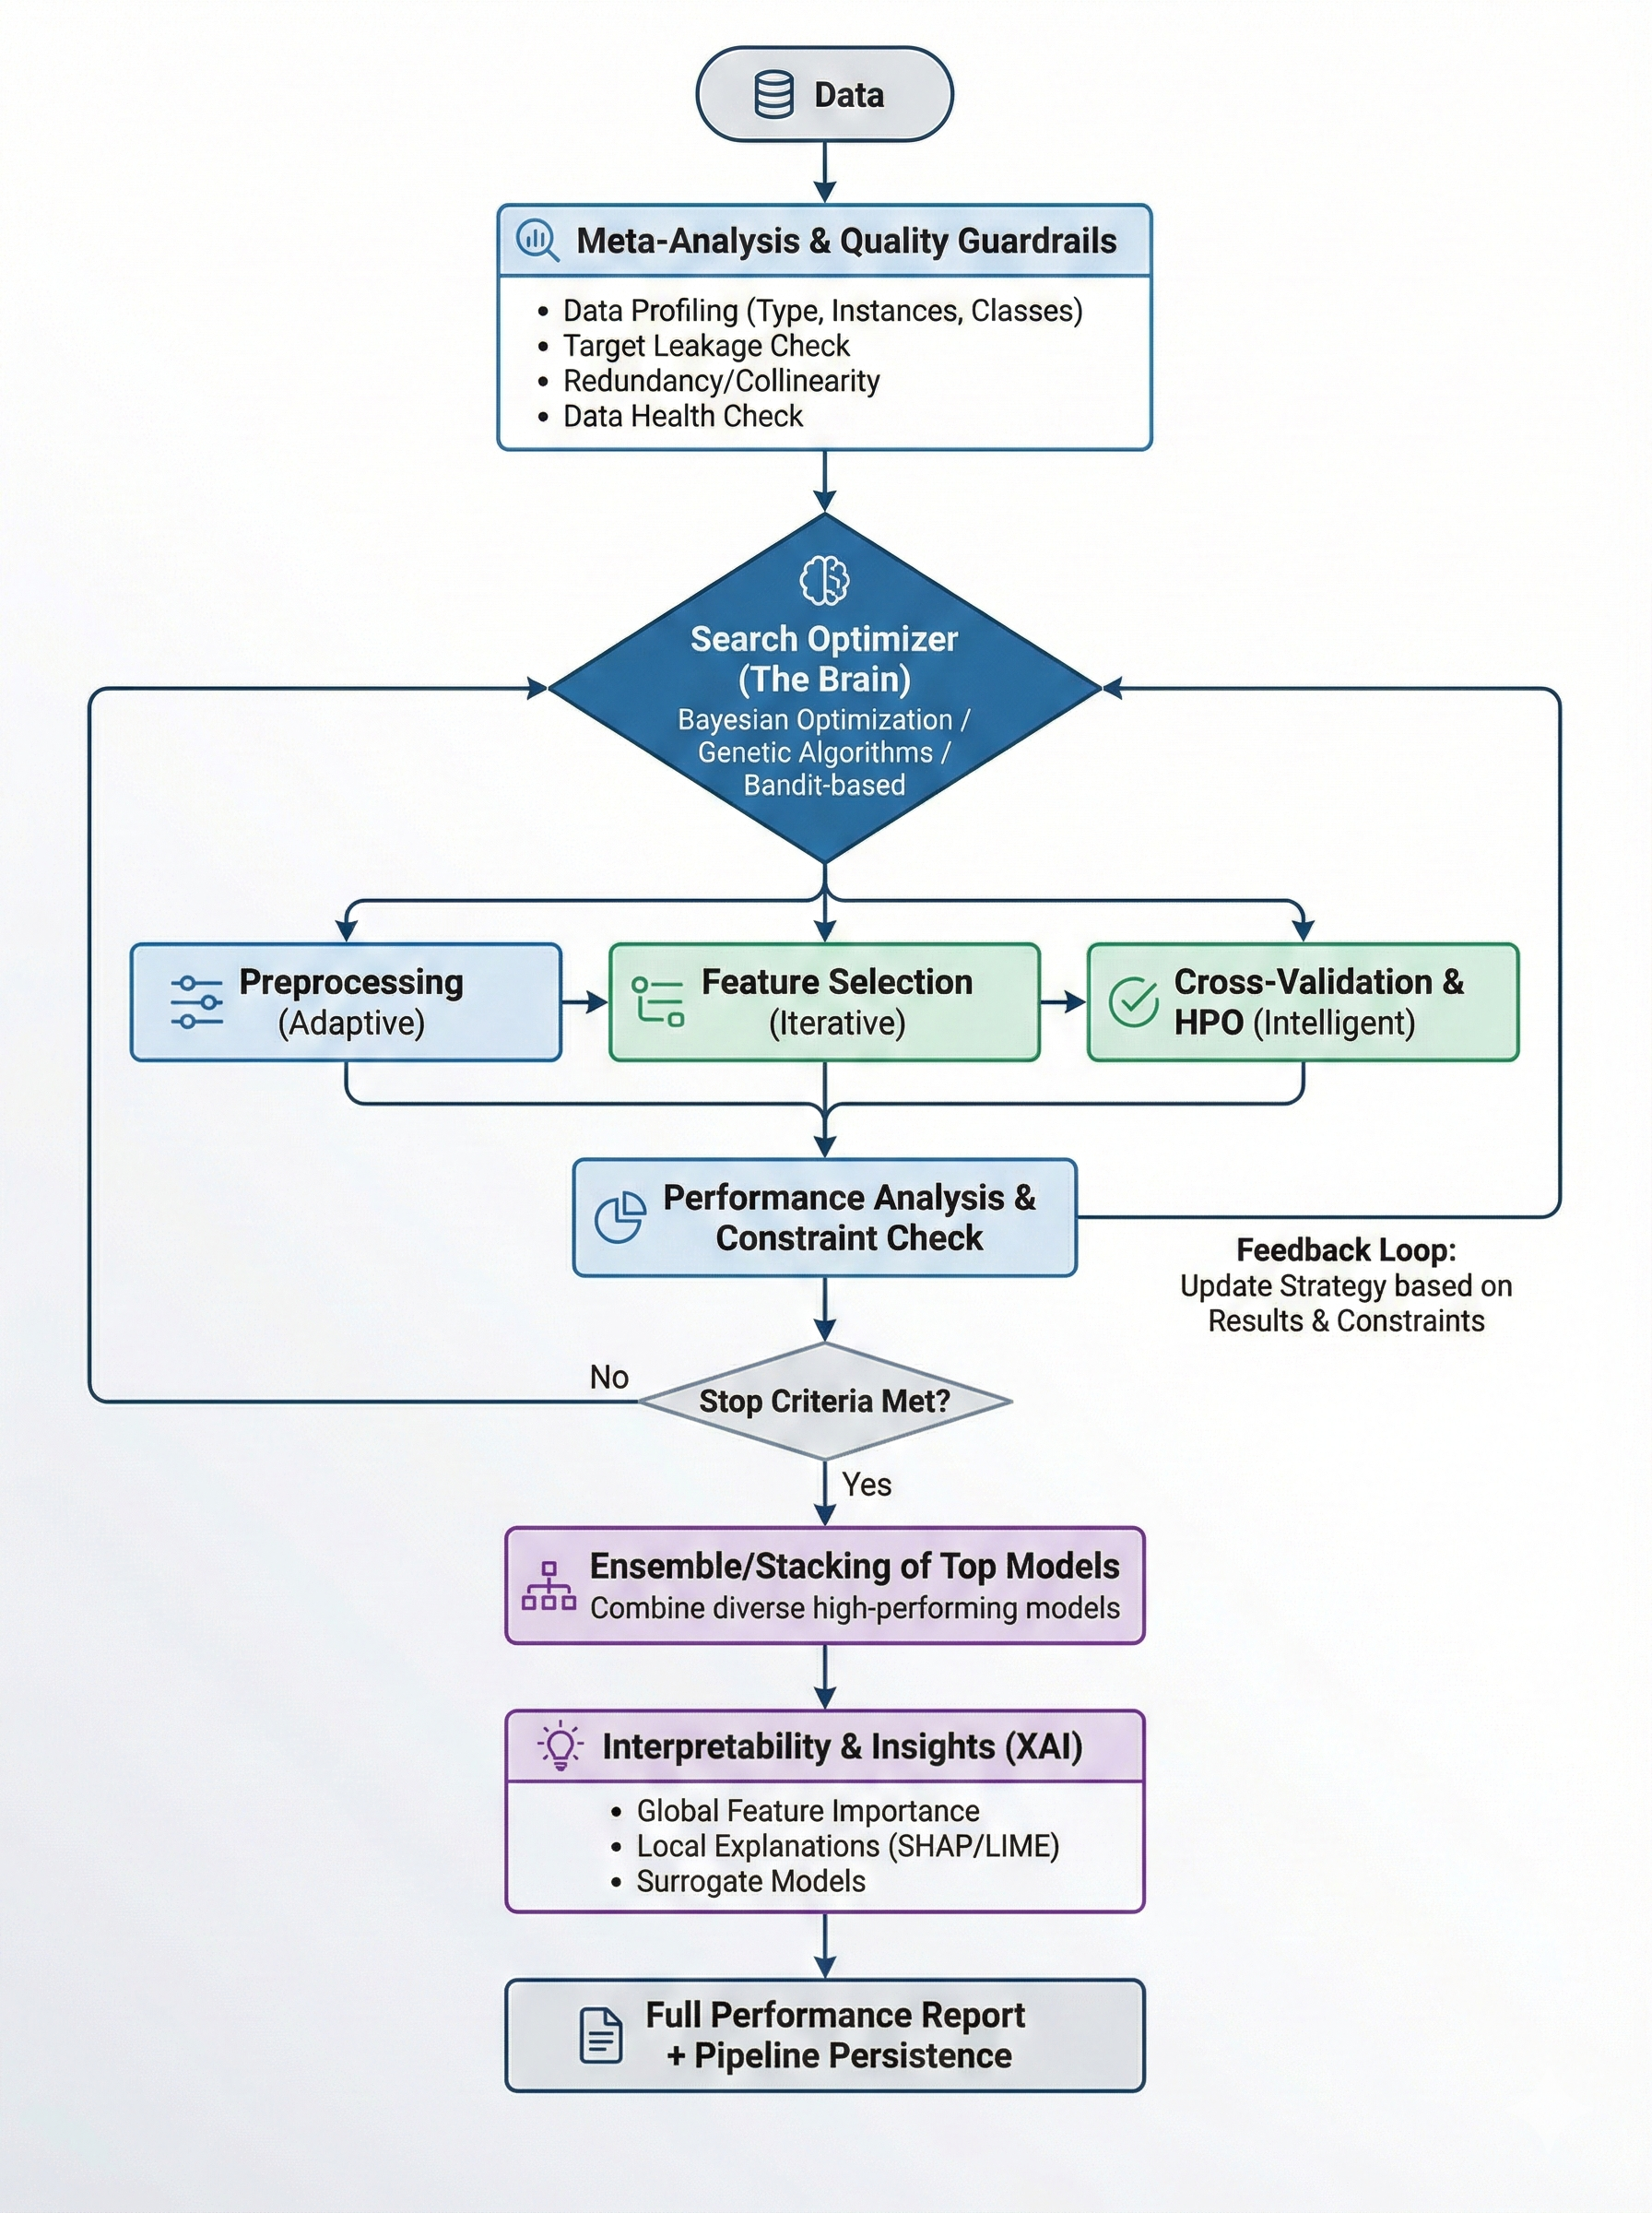
\includegraphics[width=0.90\columnwidth]{figures/endgame_automl.png}
\caption{AutoML pipeline architecture. The orchestrator manages 15 stages
  with dynamic time-budget reallocation: profiling, guardrails, baseline
  training, feature selection, HPO, ensembling, calibration, constraint
  checking, and explainability.}
\label{fig:automl}
\end{figure}

\paragraph{Signal processing.} A complete pipeline from filtering
(Butterworth, FIR, Savitzky--Golay) through spectral analysis (Welch PSD,
multitaper), wavelet decomposition (CWT, DWT, packets), to complexity
measures (permutation entropy, Higuchi fractal dimension, DFA)---all
as sklearn-compatible transformers.

\subsection{LLM Integration via MCP}

Endgame ships a Model Context Protocol server that allows any compatible
LLM host (Claude Code, Claude Desktop, VS~Code Copilot) to build ML
pipelines through natural language. Rather than exposing every component as
a separate tool---which would be token-prohibitive---the server provides a
smaller set of meta-tools grouped by workflow stage (data loading, model
discovery, training, evaluation, visualization, export), along with
browsable resources for zero-cost discovery of available models, presets,
and chart types. A \texttt{SessionManager} maintains stateful artifact
tracking across tool calls, enabling multi-turn conversational workflows
that culminate in an exportable Python script reproducing the full pipeline.

\FloatBarrier
%% --------------------------------------------------------------------------
\section{Evaluation}
\label{sec:evaluation}

We evaluate five capabilities that distinguish Endgame from existing
frameworks: (1)~interpretable models under a single API with statistical
benchmarking, (2)~LLM-driven pipeline construction via the built-in MCP
server, (3)~unified calibration, fairness, and validation support,
(4)~production AutoML with quality guardrails, and (5)~developer ergonomics.

\subsection{Interpretable Model Zoo}
\label{sec:eval:glassbox}

A central design goal of Endgame is making glass-box models first-class
citizens. The framework provides 33 interpretable models spanning 9
paradigms---generalized additive models (EBM, pyGAM, GAMI-Net, NODE-GAM,
NAM), optimal rule lists (CORELS, GOSDT), integer risk scorecards (SLIM,
FasterRisk), rule ensembles (RuleFit), fuzzy rules (FURIA), symbolic
regression (PySR), decision rules (C5.0 via a custom Rust backend),
piecewise linear models (MARS), and Bayesian network classifiers (TAN, KDB,
ESKDB). All share the same \texttt{fit}/\texttt{predict} interface as
black-box models, enabling direct comparison within a single experiment.

To illustrate, we train five glass-box models from different paradigms on
the Heart Disease dataset (270 patients, 13 clinical features, binary
classification)---using identical code for each:

\begin{lstlisting}
import endgame as eg
from sklearn.datasets import fetch_openml

data = fetch_openml(data_id=53, as_frame=True)
X, y = data.data, data.target
models = {
    "EBM":     eg.models.EBMClassifier(),
    "C5.0":    eg.models.C50Classifier(),
    "RuleFit": eg.models.RuleFitClassifier(),
    "MARS":    eg.models.MARSClassifier(),
    "TAN":     eg.models.TANClassifier(),
}
for name, m in models.items():
    m.fit(X_train, y_train)
\end{lstlisting}

\noindent Each model learns a qualitatively different representation of the
same data: the EBM discovers per-feature shape functions---e.g., heart
disease risk increasing sharply with age above 55
(Figure~\ref{fig:glassbox}a)---while RuleFit extracts clinically readable
rules like ``\texttt{IF cholesterol > 250 AND max\_heart\_rate < 140}'' (b).
TAN learns a Bayesian network encoding feature dependencies (c), and MARS
fits piecewise linear hinge functions on clinical variables (d). After
training, the learned structures are accessible programmatically (e.g.,
\texttt{ebm.get\_histogram()}, \texttt{rulefit.get\_rules()},
\texttt{tan.structure\_}), enabling downstream auditing and domain-expert
review.

\begin{figure}[!htb]
\centering
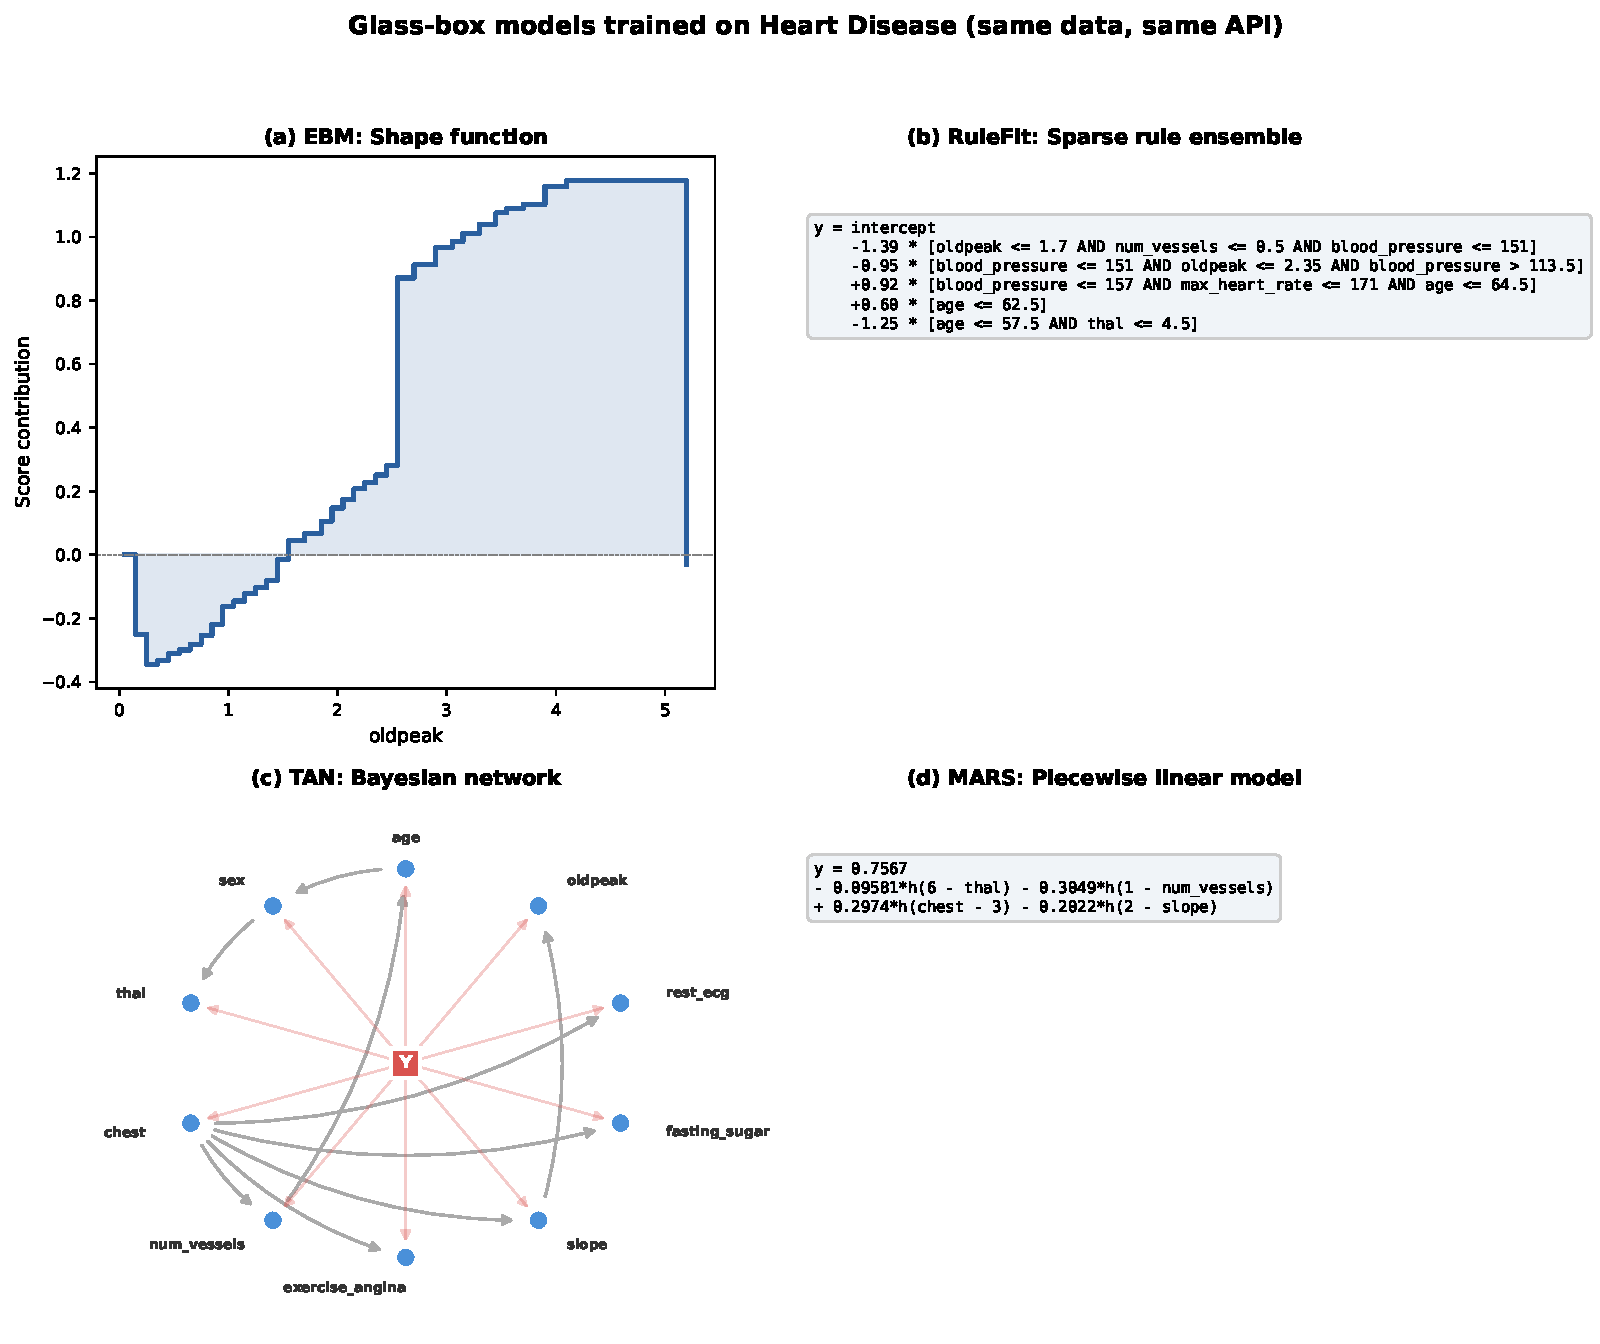
\includegraphics[width=\columnwidth]{figures/glassbox_showcase.pdf}
\caption{Glass-box models trained on the Heart Disease dataset with the
  same API, each learning a qualitatively different interpretable
  representation from 13 clinical features.}
\label{fig:glassbox}
\end{figure}

Table~\ref{tab:glassbox} compares accuracy across 29 benchmark datasets
using default hyperparameters. Glass-box models such as EBM achieve accuracy
on par with LightGBM while remaining fully interpretable, and the Friedman
test confirms significant accuracy differences across models. Several
models---C5.0 (Rust backend), TAN, ESKDB, RuleFit---are unavailable in any
other unified framework.

\begin{table}[!htb]
\centering
\caption{Glass-box vs.\ black-box accuracy across 29 benchmark datasets (mean $\pm$ std over per-dataset accuracy). All models use default hyperparameters. Friedman test across 12 models with $\geq$20 datasets on 22 shared datasets: $\chi^2 = 117.2$, $p < 0.001$.}
\label{tab:glassbox}
\small
\begin{tabular}{@{}llccc@{}}
\toprule
\textbf{Model} & \textbf{Paradigm} & \textbf{Datasets} & \textbf{Mean Acc.} & \textbf{Unique} \\
\midrule
\multicolumn{5}{l}{\textit{Glass-box (interpretable)}} \\
EBM & Additive (GAM) & 28 & $0.883 \pm 0.110$ & \checkmark \\
MARS & Piecewise linear & 28 & $0.793 \pm 0.133$ & \checkmark \\
RuleFit & Rule ensemble & 10 & $0.928 \pm 0.113$ & \checkmark \\
C5.0 & Decision rules (Rust) & 28 & $0.824 \pm 0.115$ & \checkmark \\
TAN & Bayesian network & 23 & $0.853 \pm 0.108$ & \checkmark \\
ESKDB & Bayesian ensemble & 22 & $0.836 \pm 0.111$ & \checkmark \\
NAM & Neural additive & 28 & $0.821 \pm 0.145$ & \checkmark \\
NaiveBayes & Probabilistic & 28 & $0.758 \pm 0.157$ &  \\
\midrule
\multicolumn{5}{l}{\textit{Black-box (reference)}} \\
LightGBM & GBDT & 28 & $0.883 \pm 0.118$ & \\
CatBoost & GBDT & 28 & $0.886 \pm 0.112$ & \\
XGBoost & GBDT & 28 & $0.877 \pm 0.117$ & \\
RandomForest & Ensemble & 29 & $0.878 \pm 0.112$ & \\
FT-Transformer & Deep tabular & 28 & $0.766 \pm 0.188$ & \\
\bottomrule
\end{tabular}
\end{table}

\subsection{LLM-Driven Pipeline Construction via MCP}
\label{sec:eval:mcp}

Endgame ships a Model Context Protocol (MCP) server that enables any
compatible LLM host---Claude Code, Claude Desktop, VS~Code Copilot---to
build complete ML pipelines through natural language conversation. Rather
than exposing each of the 97+ models as a separate tool (which would consume
the LLM's context window), the server provides 20 meta-tools organized by
workflow stage and 6 browsable resources for zero-cost model discovery
(Figure~\ref{fig:mcp}).

\begin{figure}[!htb]
\centering
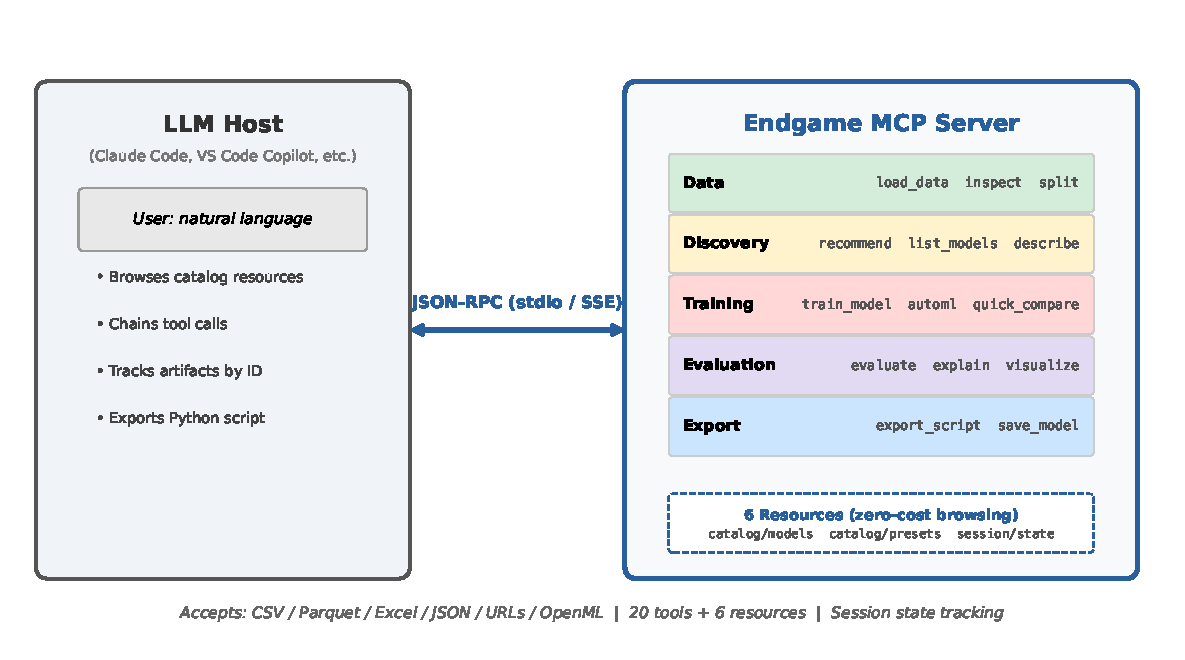
\includegraphics[width=\columnwidth]{figures/mcp_flow.pdf}
\caption{MCP server architecture. The \texttt{load\_data} tool accepts
  CSV, Parquet, Excel, JSON, URLs, and OpenML sources. A
  \texttt{SessionManager} tracks artifacts across turns, enabling
  multi-step pipelines that culminate in an exportable Python script.}
\label{fig:mcp}
\end{figure}

The server accepts any tabular data source---not just canned benchmarks.
A user can point to a local CSV, a Parquet file, a URL, or an OpenML dataset:

\begin{lstlisting}[numbers=none]
# Load from a local file
load_data(source="patients.csv",
          target_column="diagnosis")
# Load from a URL
load_data(source="https://hospital.org/data.parquet",
          target_column="readmitted")
# Load from OpenML
load_data(source="openml:diabetes",
          target_column="class")
\end{lstlisting}

\noindent Once data is loaded, the LLM chains tool calls through a
stateful session. A typical multi-turn workflow:

\begin{lstlisting}[numbers=none]
# 1. Load and inspect
load_data(source="clinic_data.csv",
          target_column="heart_disease")
inspect_data(dataset_id="ds_7f2a")

# 2. Train interpretable models
train_model(model_name="ebm", cv_folds=5)
train_model(model_name="rulefit", cv_folds=5)

# 3. Evaluate and explain
evaluate_model(model_id="model_a1b2")
explain_model(model_id="model_a1b2",
              method="importance")

# 4. Export reproducible script
export_script(model_id="model_a1b2",
              include_preprocessing=True)
\end{lstlisting}

\noindent This design solves a key challenge in LLM--tool integration: the
schema for 20 meta-tools fits in under 2K tokens, whereas exposing
individual model constructors would require 50K+ tokens.

\subsection{Calibration, Fairness, and Validation}
\label{sec:eval:calibration}

Endgame provides first-class support for the production requirements that
typically require separate libraries.

\paragraph{Calibration and conformal prediction.} Any classifier can be
wrapped in a conformal predictor or probability calibrator with a single
line:

\begin{lstlisting}[numbers=none]
from endgame.calibration import ConformalClassifier
from endgame.calibration import VennABERS

# Conformal prediction sets (coverage guarantee)
conf = ConformalClassifier(model, method="lac")
conf.fit(X_train, y_train, X_cal, y_cal)
sets = conf.predict_set(X_test, alpha=0.05)

# Venn-ABERS calibrated probabilities
va = VennABERS(model)
va.fit(X_cal, y_cal)
p_low, p_high = va.predict_proba(X_test)
\end{lstlisting}

\noindent Six calibration methods (Platt, isotonic, beta, Venn-ABERS,
temperature, histogram binning) share a common interface and can be
compared via Expected Calibration Error.

\paragraph{Fairness auditing and mitigation.} The \texttt{fairness} module
provides demographic parity, equalized odds, disparate impact, and
calibration-by-group metrics, along with three mitigation strategies:

\begin{lstlisting}[numbers=none]
from endgame.fairness import (
    demographic_parity, equalized_odds,
    ReweighingPreprocessor,
    ExponentiatedGradient)

# Audit
dp = demographic_parity(y_true, y_pred,
                        sensitive=gender)
eo = equalized_odds(y_true, y_pred,
                    sensitive=gender)

# Mitigate via sample reweighing
rw = ReweighingPreprocessor(sensitive_col="gender")
X_rw, weights = rw.fit_transform(X, y)
\end{lstlisting}

\paragraph{Validation strategies.} Beyond standard $k$-fold,
Endgame provides 8 cross-validation strategies tailored to specific data
structures: \texttt{PurgedTimeSeriesSplit} with embargo for financial
backtesting, \texttt{StratifiedGroupKFold} for medical data with patient
IDs, \texttt{CombinatorialPurgedKFold} for combinatorial purged
cross-validation, and \texttt{AdversarialValidator} for detecting
train/test distribution shift.

\subsection{AutoML with Production Guardrails}
\label{sec:eval:automl}

The AutoML module (Figure~\ref{fig:automl}) orchestrates a 15-stage
pipeline that goes beyond the standard train--evaluate--ensemble loop with
stages absent from most AutoML systems:

\begin{enumerate}
\item \textbf{Quality guardrails} detect target leakage (feature--target
  correlation $>0.95$), redundant features, extreme class imbalance, and
  data health issues \emph{before} any model is trained. In strict mode,
  critical issues abort the pipeline.

\item \textbf{Deployment constraints} filter candidate models during
  training---not post-hoc---against user-specified latency, model size,
  memory, and interpretability requirements.

\item \textbf{Calibration selection} automatically compares six calibration
  methods (Platt, isotonic, beta, Venn-ABERS, temperature, histogram
  binning) via 3-fold CV on Expected Calibration Error, selecting the best.

\item \textbf{Conformal prediction} wraps the final model with
  distribution-free coverage guarantees (LAC for classification, adaptive
  intervals for regression).
\end{enumerate}

\noindent Six presets control the quality--speed trade-off, from
\texttt{fast} (5 minutes, single LightGBM) to \texttt{best\_quality}
(unlimited, full model pool with 100 HPO trials and stacking). A dedicated
\texttt{interpretable} preset restricts the candidate pool to glass-box
models.

\subsection{Developer Ergonomics}
\label{sec:eval:ergonomics}

A practical consequence of API unification is reduced integration overhead.
Figure~\ref{fig:loc} compares lines of code for three common workflows in
Endgame versus a standard multi-library stack (LightGBM + InterpretML +
mlens + MAPIE). Endgame reduces boilerplate by 77--93\%, primarily by
eliminating library-specific import, preprocessing, and adapter code.

\begin{figure}[!htb]
\centering
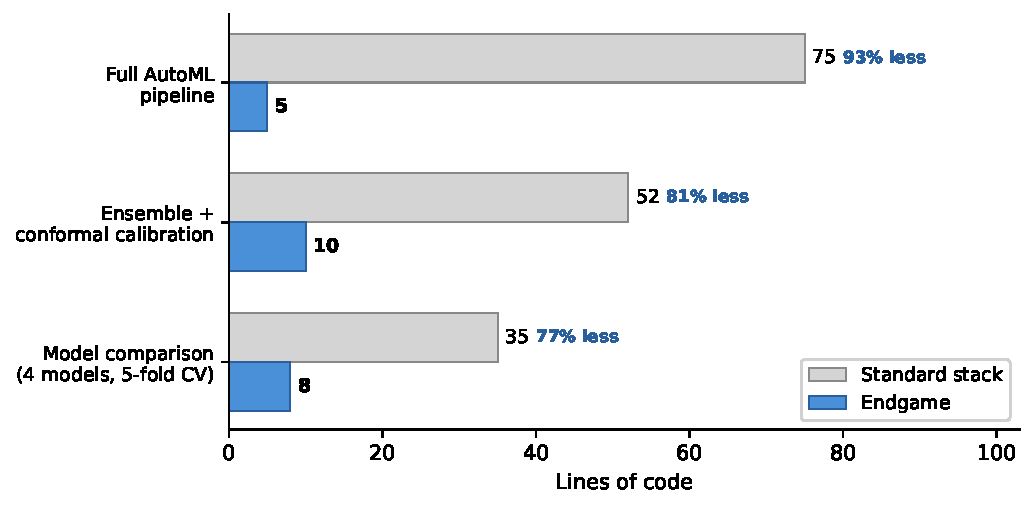
\includegraphics[width=\columnwidth]{figures/loc_comparison.pdf}
\caption{Lines of code for three common ML workflows. Endgame's unified API
  eliminates library-specific glue code.}
\label{fig:loc}
\end{figure}

\FloatBarrier
%% --------------------------------------------------------------------------
\section{Comparison with Related Software}
\label{sec:comparison}

\begin{table}[!htb]
\centering
\caption{Capability comparison with related toolkits. \checkmark\ indicates
  support; --- indicates absent or minimal support.}
\label{tab:comparison}
\small
\begin{tabular}{@{}lcccc@{}}
\toprule
\textbf{Capability} & \textbf{Endgame} & \textbf{sklearn} & \textbf{AutoGluon} & \textbf{PyCaret} \\
\midrule
Full sklearn API       & \checkmark & \checkmark & Partial    & Partial \\
Glass-box models       & 33         & ---        & 1 (EBM)    & --- \\
Deep tabular models    & \checkmark & ---        & \checkmark & --- \\
Conformal prediction   & \checkmark & ---        & ---        & --- \\
Probability calibration & 6 methods & ---        & ---        & --- \\
Fairness auditing      & \checkmark & ---        & ---        & --- \\
Signal processing      & \checkmark & ---        & ---        & --- \\
Ensemble optimization  & \checkmark & Basic      & \checkmark & Basic \\
AutoML guardrails      & \checkmark & ---        & ---        & --- \\
Deployment constraints & \checkmark & ---        & Partial    & --- \\
LLM integration (MCP)  & \checkmark & ---        & ---        & --- \\
\bottomrule
\end{tabular}
\end{table}

Scikit-learn \citep{pedregosa2011sklearn} provides the foundational API that
Endgame extends. Endgame does not aim to replace sklearn but to complement
it with model families (deep tabular, interpretable glass-box, Bayesian
network classifiers), calibration methods (conformal prediction, Venn-ABERS),
and domain-specific modules that sklearn does not ship.

AutoGluon \citep{erickson2020autogluon} excels at AutoML for tabular data
with sophisticated multi-layer stacking and automated model selection.
Endgame's AutoML pipeline differs in emphasis: it adds pre-training quality
guardrails (leakage detection, data health checks), deployment constraint
filtering during training rather than post-hoc, and automatic calibration
selection. Endgame also provides strict sklearn API compatibility, enabling
composition with arbitrary sklearn pipelines, and a broader interpretable
model suite (CORELS, GOSDT, SLIM, symbolic regression, fuzzy rules---in
addition to EBM). AutoGluon provides more mature ensemble selection.

H2O AutoML \citep{ledell2020h2o} provides a scalable AutoML engine with
distributed training and a Java-based backend. It excels at large-scale
deployments but does not offer interpretable model families beyond basic
decision trees, conformal prediction, or sklearn API compatibility.

Ludwig \citep{molino2019ludwig} offers a declarative, configuration-driven
approach to building deep learning pipelines. It emphasizes ease of use for
neural architectures but does not target the breadth of classical and
interpretable methods that Endgame provides.

PyCaret provides a low-code interface for common ML tasks with a streamlined
exploratory workflow. Endgame provides deeper support for uncertainty
quantification, interpretable models, custom ensemble strategies, and
signal processing.

Endgame ships a built-in MCP server, enabling LLM agents to use the full
library through natural language without additional glue code---a
capability not currently available in the toolkits listed above.

%% --------------------------------------------------------------------------
\section{Target Use Cases}
\label{sec:usecases}

Endgame is designed for four primary settings.

\emph{Research benchmarking}: the unified API enables fair comparison across
model families (e.g., deep tabular vs.\ interpretable vs.\ ensemble) without
confounds introduced by differing preprocessing or evaluation code.

\emph{Regulated and high-stakes domains}: healthcare applications requiring
interpretable models for clinical decision support, financial services
needing calibrated probabilities and auditable pipelines, and insurance
underwriting with fairness constraints. The co-location of glass-box models,
conformal prediction, and fairness metrics under one framework simplifies
regulatory compliance.

\emph{Applied industry verticals}: predictive maintenance for home services
and manufacturing (combining signal processing with supervised learning),
supply chain forecasting for wholesale and logistics (time series modules
with conformal intervals), and automated valuation models for real estate
(interpretable models with calibrated uncertainty). These verticals benefit
from Endgame's domain-specific modules and the ability to move from
prototype to production within a single framework.

\emph{Competition and rapid prototyping}: competition-tuned presets, the
AutoML pipeline, and the Quick API (\texttt{classify}, \texttt{compare})
provide fast baselines with minimal boilerplate.

%% --------------------------------------------------------------------------
\section{Limitations}
\label{sec:limitations}

Endgame prioritizes breadth of coverage over deep specialization in any
single domain. For example, its vision and NLP modules provide useful
wrappers around timm and HuggingFace Transformers, but do not attempt to
match the feature depth of domain-specific frameworks like Detectron2 or
spaCy. The broad scope carries a maintenance burden: keeping 97+ model
wrappers current as upstream libraries evolve requires ongoing effort, and
some wrappers may lag behind the latest releases of their backends. The full
installation carries a substantial dependency footprint; optional dependency
groups mitigate this, but users working in constrained environments should
install only the modules they need. The current benchmark covers 29 datasets
from the sklearn-classic and OpenML suites; extending to
TabZilla \citep{mcelfresh2024neural} (176 datasets) and full OpenML-CC18 is
planned, along with direct runtime and accuracy comparisons against
AutoGluon, H2O, and PyCaret.

%% --------------------------------------------------------------------------
\section{Installation and Usage}
\label{sec:usage}

Endgame requires Python 3.10+ and is installable via pip:

\begin{verbatim}
pip install endgame-ml            # core
pip install endgame-ml[tabular]   # + GBDTs, deep tabular, EBM
pip install endgame-ml[all]       # all optional dependencies
\end{verbatim}

\noindent Documentation and examples are available at
\url{https://github.com/allianceai/endgame}.

%% --------------------------------------------------------------------------
\section{Conclusion and Future Work}
\label{sec:conclusion}

Endgame provides a unified, scikit-learn-compatible framework that brings
together classic and modern methods from across machine learning. Its primary
contribution is making interpretable and calibrated models first-class
citizens: the framework's 33 glass-box models across 9 paradigms enable
direct comparison of accuracy--interpretability trade-offs within a single
experiment---a workflow that is impractical when these models are scattered
across separate libraries. The built-in MCP server provides native LLM
integration for pipeline construction, and the 15-stage AutoML pipeline adds
production guardrails absent from most AutoML systems. Benchmarking across
29 datasets confirms that glass-box models such as EBM achieve accuracy on
par with gradient boosted trees while remaining fully interpretable.

Future work includes extending benchmarks to TabZilla (176 datasets) and
OpenML-CC18 with direct comparisons against AutoGluon and H2O,
multi-objective optimization in the AutoML module, and continued integration
of emerging methods. The software is actively maintained, released under the
Apache~2.0 license, and available at
\url{https://github.com/allianceai/endgame}.

%% --------------------------------------------------------------------------
\bibliographystyle{plainnat}

\begin{thebibliography}{20}

\bibitem[Angelino et~al.(2017)]{angelino2017learning}
Elaine Angelino, Nicholas Larus-Stone, Daniel Alabi, Margo Seltzer, and
  Cynthia Rudin.
\newblock Learning certifiably optimal rule lists for categorical data.
\newblock \emph{Journal of Machine Learning Research}, 18(234):1--78, 2017.

\bibitem[Anthropic(2024)]{anthropic2024mcp}
Anthropic.
\newblock Model Context Protocol specification.
\newblock \url{https://modelcontextprotocol.io/}, 2024.

\bibitem[Cranmer(2023)]{cranmer2023interpretable}
Miles Cranmer.
\newblock Interpretable machine learning for science with {PySR} and
  {SymbolicRegression.jl}.
\newblock \emph{arXiv preprint arXiv:2305.01582}, 2023.

\bibitem[Dem\v{s}ar(2006)]{demsar2006statistical}
Janez Dem\v{s}ar.
\newblock Statistical comparisons of classifiers over multiple data sets.
\newblock \emph{Journal of Machine Learning Research}, 7:1--30, 2006.

\bibitem[Erickson et~al.(2020)]{erickson2020autogluon}
Nick Erickson, Jared Mueller, Alexander Shirkov, Hang Zhang, Pedro Larroy,
  Mu~Li, and Alexander Smola.
\newblock Auto{G}luon-{T}abular: Robust and accurate {AutoML} for structured
  data.
\newblock \emph{arXiv preprint arXiv:2003.06505}, 2020.

\bibitem[Gorishniy et~al.(2021)]{gorishniy2021revisiting}
Yury Gorishniy, Ivan Rubachev, Valentin Khrulkov, and Artem Babenko.
\newblock Revisiting deep learning models for tabular data.
\newblock In \emph{Advances in Neural Information Processing Systems (NeurIPS)}, 2021.

\bibitem[Gorishniy et~al.(2024)]{gorishniy2024tabr}
Yury Gorishniy, Ivan Rubachev, and Artem Babenko.
\newblock Tab{R}: Tabular deep learning meets nearest neighbors in 2024.
\newblock In \emph{International Conference on Learning Representations (ICLR)}, 2024.

\bibitem[LeDell and Poirier(2020)]{ledell2020h2o}
Erin LeDell and Sebastien Poirier.
\newblock {H2O} {AutoML}: Scalable automatic machine learning.
\newblock In \emph{ICML AutoML Workshop}, 2020.

\bibitem[Hollmann et~al.(2023)]{hollmann2022tabpfn}
Noah Hollmann, Samuel M{\"u}ller, Katharina Eggensperger, and Frank Hutter.
\newblock Tab{PFN}: A transformer that solves small tabular classification
  problems in a second.
\newblock In \emph{International Conference on Learning Representations (ICLR)}, 2023.

\bibitem[Lin et~al.(2020)]{lin2020generalized}
Jimmy Lin, Chudi Zhong, Diane Hu, Cynthia Rudin, and Margo Seltzer.
\newblock Generalized and scalable optimal sparse decision trees.
\newblock In \emph{International Conference on Machine Learning (ICML)}, 2020.

\bibitem[Liu and Rudin(2022)]{liu2022fasterrisk}
Jiachang Liu and Cynthia Rudin.
\newblock {FasterRisk}: Fast and accurate interpretable risk scores.
\newblock In \emph{Advances in Neural Information Processing Systems (NeurIPS)}, 2022.

\bibitem[Molino et~al.(2019)]{molino2019ludwig}
Piero Molino, Yaroslav Dudin, and Sai~Sumanth Miryala.
\newblock Ludwig: a type-based declarative deep learning toolbox.
\newblock \emph{arXiv preprint arXiv:1909.07930}, 2019.

\bibitem[McElfresh et~al.(2024)]{mcelfresh2024neural}
Duncan McElfresh, Sujay Khandagale, Jonathan Valverde, Vishak Prasad C.,
  Ganesh Ramakrishnan, Micah Goldblum, and Colin White.
\newblock When do neural nets outperform boosted trees on tabular data?
\newblock In \emph{Advances in Neural Information Processing Systems (NeurIPS)}, 2024.

\bibitem[Marton et~al.(2024)]{marton2024grande}
Sascha Marton, Stefan L{\"u}dtke, Christian Bartelt, and Heiner Stuckenschmidt.
\newblock {GRANDE}: Gradient-based decision tree ensembles for tabular data.
\newblock In \emph{International Conference on Learning Representations (ICLR)}, 2024.

\bibitem[Nori et~al.(2019)]{nori2019interpretml}
Harsha Nori, Samuel Jenkins, Paul Koch, and Rich Caruana.
\newblock Interpret{ML}: A unified framework for machine learning
  interpretability.
\newblock \emph{arXiv preprint arXiv:1909.09223}, 2019.

\bibitem[Pedregosa et~al.(2011)]{pedregosa2011sklearn}
Fabian Pedregosa, Ga{\"e}l Varoquaux, Alexandre Gramfort, Vincent Michel,
  Bertrand Thirion, Olivier Grisel, Mathieu Blondel, Peter Prettenhofer,
  Ron Weiss, Vincent Dubourg, et~al.
\newblock Scikit-learn: Machine learning in {P}ython.
\newblock \emph{Journal of Machine Learning Research}, 12:2825--2830, 2011.

\bibitem[Popov et~al.(2020)]{popov2020neural}
Sergei Popov, Stanislav Morozov, and Artem Babenko.
\newblock Neural oblivious decision ensembles for deep learning on tabular
  data.
\newblock In \emph{International Conference on Learning Representations (ICLR)}, 2020.

\bibitem[Romano et~al.(2019)]{romano2019conformalized}
Yaniv Romano, Evan Patterson, and Emmanuel Cand\`{e}s.
\newblock Conformalized quantile regression.
\newblock In \emph{Advances in Neural Information Processing Systems (NeurIPS)}, 2019.

\bibitem[Somepalli et~al.(2021)]{somepalli2021saint}
Gowthami Somepalli, Micah Goldblum, Avi Schwarzschild, C.~Bayan Bruss, and
  Tom Goldstein.
\newblock {SAINT}: Improved neural networks for tabular data via row attention
  and contrastive pre-training.
\newblock \emph{arXiv preprint arXiv:2106.01342}, 2021.

\bibitem[van~der Laan et~al.(2007)]{van2007super}
Mark~J. van~der Laan, Eric~C. Polley, and Alan~E. Hubbard.
\newblock Super learner.
\newblock \emph{Statistical Applications in Genetics and Molecular Biology},
  6(1), 2007.

\end{thebibliography}

\end{document}
